\chapter{Introduction}
	\label{sec:Introduction} 
	
	\section{Introduction}
		\label{}
		The rapid development of Internet technology has provided unprecedented convenience and efficiency for people, and the dependence on transportation in daily life is ever-growing. At present, all countries are making efforts to develop intelligent urban transportation. The Internet of Vehicles is the inevitable trend of future development. Internet of Vehicles (IoV) is a concrete manifestation of the Internet of Things (IoT) in the field of vehicles. Through vehicle-related technologies and equipment, attributes and information of all vehicles, pedestrians and road infrastructure in the network are effectively identified, and data are integrated on the back-end platform for intelligent management and service. \\
		ITS in Europe and Japan have adopted certain forms of IoV technology. In New Delhi, all $55,000$ licensed rickshaws have been fitted with GPS devices so that drivers can be held accountable for their questionable route selection. China’s Ministry of Transport had ordered that GPS systems be installed and connected on all long-haul buses and Hazmat vehicles by the end of 2011, to ensure good driving habits and reduce the risk of accidents and traffic jam. The Brazilian government has set a goal for all cars in circulation to be fitted with electronic ID chips from its National Automated Vehicle Identification System. \\
		More and more efforts are being made on research and development of vehicle intelligence. Almost all major vehicle manufactures have started their intelligent-vehicle projects, including Toyota, Ford, GM, BMW, Volvo, etc. Also, major IT corporations such as Google, Apple, Baidu, and Huawei are working on intelligent-vehicle systems. 
	
	\section{Problem Statement}
		\label{}
		Due to the particularity of the Internet of Vehicles system service, vehicles need to broadcast their sensitive information such as location and identity information frequently. Attackers can collect and analyze vehicle broadcast information to steal privacy and even directionally track the owner through the driving trajectory, bringing serious security risks. Also, avoiding single point of failure of traditional approach due to centralized systems is one of our critical concerns. 
		
	\section{Motivations}
		\label{}
		The concept of IoV has been recognized by more and more people in recent years, and it is currently in a stage of evolving from concept to reality. The number of vehicles in vehicular networks is constantly rising and may cross two billion within the next 10-20 years. IoV is critical for realizing this number and to facilitate next-generation intelligent transportation systems (ITS) and related technologies. One of the primary IoV objectives is to enhance traffic efficiency and improve the safety of vehicles, its passengers, and the pedestrians alike. According to World Health Organization (WHO), traffic accidents account for approximately $1.25$ million deaths every year. Therefore, trust management protocols in IoV are needed to guarantee road safety measures. Besides, the environments of IoV could be dangerous in the absence of security protections. Due to the openness and self-organization of Internet of Vehicles, there are enormous malicious attackers. Malicious entities can compromise a vehicle, which not only endangers the security of the vehicle but also the safety of the passengers. 
	
	\section{Project Aim}
		\label{}
		Our purpose is to guarantee security targets such as confidentiality, integrity, and availability in our system. This purpose is achieved by using a block chain and certain cryptographic algorithms, this is all must be guaranteed with emphasis on reliability, scalability, and ease of use of the system. 
	
	\section{Objectives}
		\label{}
		\begin{itemize}
			\item Build the proposed system based that guarantees security communication between vehicles to vehicle and achieve confidentiality and integrity for the shared messages between them. 
			\item Evaluate the system by doing performance analysis. 
			\item Secure the system against common attacks, such as Distributed Denial of Service, Man-in-the-middle, and Replay attacks. 
			\item Validate the used security algorithms in the proposed system using formal simulation tools. 
		\end{itemize}
	
	\section{Project Scope}
		\label{}
		Designing a security solution for IoV system using Blockchain, Cryptography, and Fog computing technologies, followed by building a proof of concept in the form of simulation using OMNET++ which is an open source tool that provides an extensive library to simulate network characteristics using a set of frameworks and commonly used by researchers. 
		
	\section{Proposed Solution}
		\label{}
		We propose a privacy protection system to secure communication on the Internet of Vehicles (IOV). This system depends on blockchain to avoid data tampering and prevent the central failure problem. It also uses hybrid encryption to ensure anonymity and confidentiality of security information. 
	
	\section{Project Phases}
		\label{}
		The methodology we are using is waterfall project management methodology. The waterfall method is a traditional approach to project management. In this methodology tasks and phases are completed in a linear or sequential manner, and each stage of the project must be completed before the next begins. And as the outcome of the project is clear and already determined we saw this approach is better for our project. \\
		The stages of Waterfall project management generally follow this sequence: \\
		\begin{itemize}
			\item \textbf{Problem Identification}\\
			In this stage, we started to read different papers that explain the Internet of Vehicles (IoV) systems and security issues which they face and the resulting damage of these issues. We categorized the different problems that IoV faces and made more research to face the different kinds of problems and getting solutions to it. Then we explored the different proposed solutions to secure the IoV communications.\\
			\item \textbf{Planning}\\
			We started to determine the objectives that we aim to achieve, the needed resources to implement the different tasks. We created a time plan to decide the needed time for each phase and task then we determined the tracking and assessment methods and assigned different tasks for each member of the project team. 
			\item \textbf{Analysis}\\
			We started to check many tools and discover more technologies to build our system and explored the different proposed solutions comparing which of them is the best.  In every tool and technology, we decided to use, we see in detail each individual technologies used in the explored solutions  to understand them in a deeper level what is the benefits we get from it and what is the problems we may find in it and what to use better than it. 
			\item \textbf{Design}\\
			Based on the knowledge and experience gained from the previous phases we planned out a new architecture that meets the requirements. Means of implementing the project solution are defined. \\
			We started to build the structure of our system, actors, security protocols and how they interact with each other to achieve the goal of the system. 
			\item \textbf{Implementation}\\
			In this phase, we built the solution which we designed in the previous phase and put all of the knowledge that we have learnt to avoid the problems that we had seen in explored papers and research. 
			\item \textbf{Testing}\\
			After designing and building the proposed system including security protocols and the process of interaction of actors with each other, we have started this phase  in which we use AVISPA tool for testing and validating the used protocols against cyber-attacks. 
			\item \textbf{Documentation}\\
			Documentation process was continuous in parallel with all previous phases taking in consideration that all mentioned details are simple and clear to be understood by junior engineers who learn about securing the IoV systems. 
		\end{itemize}
		Progress flows in one direction, like a real waterfall. Also like a real waterfall, though, this can quickly get dangerous. Since everything is mapped out at the beginning, there’s a lot of room for error if expectations don’t match up with reality. And there’s no going back to a previous stage once it’s completed (just imagine trying to swim against a waterfall — not fun). 
	
	\newpage
	\section{Project Time Plan}
		\label{}
		We assume that our project plan would follow the time plan shown in Fig. \ref{timeplan}.
		\begin{figure}[!h]
			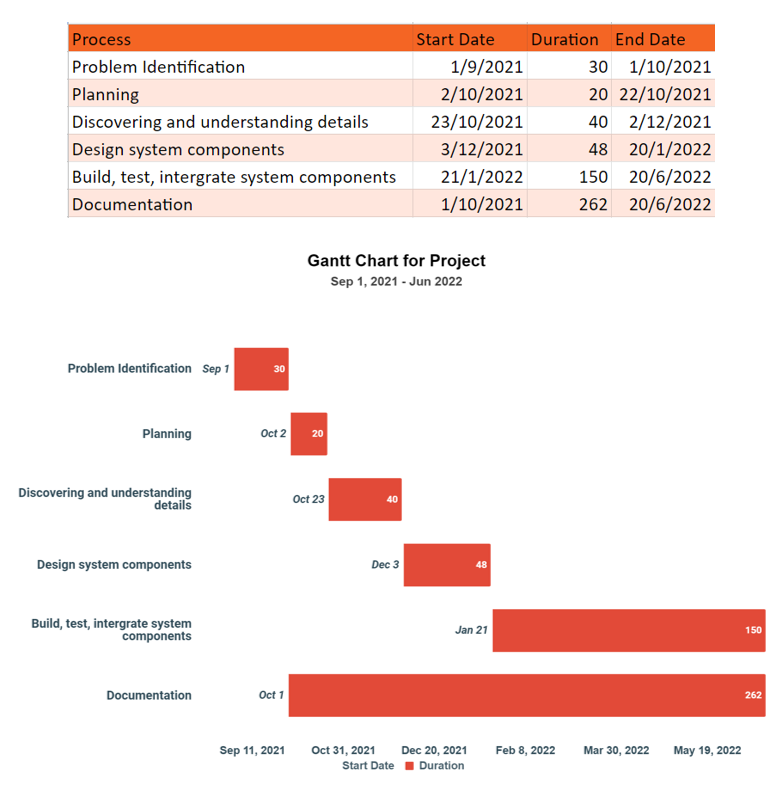
\includegraphics[width=\columnwidth]{{../images/chapter1/project_plan.png}}
			\centering
			\caption{Project Time Plan.}
			\label{timeplan}
		\end{figure}
	

